%
% DOCUMENTAZIONE PER LA REDAZIONE DEL SEGUENTE MANUALE
% STILI:
% - NOMI SOFTWARE = \newcommand{\soft}[1]{\texttt{#1}}
% - NOMI PROGETTI/LICENZA = \newcommand{\pro}[1]{\emph{#1}}
% - KEY = \newcommand{\key}[1]{\underline{\textbf{#1}}}
% - VALUE = \newcommand{\val}[1]{\underline{\textit{#1}}}
% - OpenStreetMap = \newcommand{\osm}{\emph{OpenStreetMap}\xspace}
% - GPS \newcommand{\gps}{GPS\xspace}
% - url = \url{}
%
%
%
\documentclass[a4paper,twoside,12pt,]{article}
\usepackage[a4paper,top=3cm,bottom=3cm,left=3.8cm,right=3.8cm]{geometry}
\usepackage[italian]{babel}
\usepackage{wrapfig}
\usepackage{indentfirst}
\usepackage[utf8]{inputenc}
\usepackage{graphicx}
\usepackage{booktabs}
%per creare multirow nelle tabelle
\usepackage{multirow}
%per creare il color della url
\usepackage{color}
%per cambiare colore titolo
\usepackage{titlesec}
\usepackage{xspace}
%per il layout della pagine
\usepackage{fancyhdr}


\definecolor{UrlColor}{rgb}{0,0.35,0}
\usepackage[pdftitle={Introduzione ad OpenStreetMap},pdfauthor={Luca Delucchi, Maurizio Napolitano, Alessio Zanol},colorlinks=true,citecolor=UrlColor,urlcolor=UrlColor,filecolor=UrlColor,linkcolor=UrlColor]{hyperref}
%comando per scrivere openstreetmap
\newcommand{\osm}{\emph{OpenStreetMap}\xspace}
\newcommand{\gps}{GPS\xspace}
\newcommand{\key}[1]{\textsf{\textbf{#1}}}
\newcommand{\val}[1]{\textsf{#1}}
\newcommand{\soft}[1]{\texttt{#1}}
\newcommand{\pro}[1]{\emph{#1}}

\titleformat{\section}
{\color{UrlColor}\normalfont\Large\bfseries}{\thesection}{1em}{}
\titleformat{\subsection}
{\color{UrlColor}\normalfont\large\bfseries}{\thesubsection}{1em}{}
\titleformat{\subsubsection}
{\color{UrlColor}\normalfont\normalsize\bfseries}{\thesubsubsection}{1em}{}

\rhead{Minitutorial Italiano di \osm}
%opening
\title{\begin{Large}Introduzione a \osm\end{Large}}
\date{\small{Versione Ottobre 2010}}
\author{Luca Delucchi, Maurizio Napolitano, Alessio Zanol}
\begin{document}

\maketitle
\begin{center}
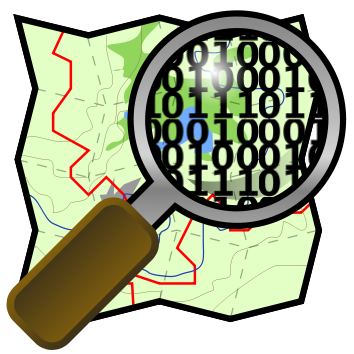
\includegraphics{Openstreetmap.png}
\end{center}
\begin{center}
	\begin{large}
	\textbf{Comunità Italiana di OpenStreetMap}
	\end{large}
\end{center}
\newpage
% \tableofcontents
% \newpage

\section{Cos'è \osm}
\osm è un progetto mondiale per la raccolta collaborativa di dati geografici da cui si possono derivare innumerevoli lavori e servizi. I risultati più evidenti sono le mappe online che però rappresentano solo la punta dell'iceberg di quel che si può ottenere da questi dati.

La \textbf{caratteristica fondamentale è che i dati di \osm possiedono una licenza libera}, attualmente è attiva una doppia licenza: la \pro{Creative Commons BY SA} che è la licenza originale del progetto che verrà sostituita con la \pro{ODbL (OpenDatabaseLicense)}, una licenza che serve a coprire i database mantenendone la libertà di utilizzo. Infatti è possibile usare i dati \osm liberamente per qualsiasi scopo, anche quelli commerciali, con il solo vincolo di citare il progetto e usare la stessa licenza per eventuali dati derivati. 

L'altra caratteristica molto importante è che tutti possono contribuire arricchendo o correggendo i dati e, come i progetti simili (\pro{Wikipedia} e mondo del software libero ad esempio) \textbf{la comunità è l'elemento fondamentale} perché oltre a essere quella che inserisce i dati e arrichisce il progetto, ne controlla anche la qualità.
\section{Cosa non è \osm}
\textbf{\osm non è una raccolta di tracce \gps tra loro slegate}. Le tracce \gps sono solo utili per capire come tracciare il reticolo delle strade e per inserire i punti di interesse.

\textbf{\osm non è una copia di Google Maps} e non è quello il suo scopo, è molto di più \dots

\section{Perché \osm}
\osm come abbiamo detto è un progetto che vuole creare una banca dati geografica libera, uno dei punti di forza è la possibilità di utilizzarla per le più svariate necessità e su  dispositivi differenti. \textbf{I dati sono disponibili in moltissimi formati}, possono essere caricati su GPS, navigatori o cellulari per sapere sempre la vostra posizione o per calcolare il percorso più breve per raggiungere una certa località; potete utilizzarli sul vostro sito per segnalare dove si trova la vostra azienda o per mostrare le vostre immagini georiferite; potete effettuare mappe cartacee a diverse scale e con diversi stili; possono essere usati come base di videogiochi; esistono in diversi formati vettoriali per essere analizzati con software GIS; per ultimo, ma forse uno dei motivi più importanti, anche se è quello per il quale si spera non debbano mai essere utilizzate, per salvare vite...

\section{La struttura del database \osm}
\subsection{Elementi}
\textbf{\osm è un database}, gli elementi che possono essere inseriti (strade, negozi, ecc.), tramite alcuni software che vedremo in seguito, sono di quattro tipologie:
\begin{itemize}
 \item 
\includegraphics{./Mf_node.png} \texttt{punti} (node): singoli punti
 \item 
\includegraphics{./Mf_way.png} \texttt{linee} (way): un insieme di punti non chiuso
 \item 
\includegraphics{./Mf_area.png} \texttt{aree} (polygon): un insieme di punti chiuso, solitamente con il tag area=yes
 \item 
\includegraphics{./Mf_relation.png} \texttt{relazioni} (relation): un insieme degli elementi precedenti, per esempio una linea degli autobus che è composta da più strade e dalle sue fermate
\end{itemize}
\subsection{Tag}
Le \textbf{etichette (tag)} servono per descrivere le caratteristiche dei vari elementi. I \textbf{tag sono sempre composti da una coppia di nomi}. Il primo è detto \key{key}, il secondo \val{value}. Solitamente la \key{key} descrive una famiglia di caratteristiche, mentre il \val{value} va più nello specifico. Ad esempio la key \key{highway} indica la famiglia delle strade di qualsiasi tipo, dalle autostrade ai sentieri. Di seguito ne presentiamo alcuni:
\begin{center}
 \begin{tabular}{ccc}
  \toprule
   \textbf{key} & \textbf{values} & \textbf{descrizione} \\
  \midrule
   \multirow{16}*{\key{highway}} 
      & \val{motorway} & autostrada \\
      & \val{trunk} & superstrada \\
      & \val{primary} & strada di importanza nazionale \\
      & \val{secondary} & strada di importanza regionale \\
      & \val{tertiary} & strada di importanza locale \\
      & \val{unclassified} & strada del reticolo di base \\
      & \val{residential} & strada per abitazioni \\
      & \val{service} & strada di servizio \\
      & \val{track} & strada agricola o forestale \\
      & \val{pedestrian} & via pedonale cittadina \\
      & \val{footway} & sentiero \\
      & \val{cycleway} & pista ciclabile \\
      & \val{steps} & scala \\
      & \val{bus\_stop} & fermata dell'autobus \\
      & \val{stop} & segnale stop \\
      & \val{traffic\_signal} & semaforo \\
  \bottomrule
 \end{tabular}
\end{center}
I tag non rappresentano solo un elemento, ma possono essere usati per più elementi: per esempio \key{highway} è prevalentemente associato alle linee ma, come potete vedere sopra, vi sono alcuni casi in cui è utilizzato con i nodi \key{highway}=\val{bus\_stop} o \key{highway}=\val{traffic\_signal}.

I tag usati sono tantissimi e continuano ad aumentare e migliorare, permettendo di mappare qualsiasi elemento possa essere rappresentato da una coppia di coordinate geografiche. Una vasta lista è disponibile al link  \url{http://wiki.openstreetmap.org/wiki/Map_Features}. Inoltre è possibile controllare, discutere e votare i nuovi tag proposti in questa pagina \url{http://wiki.openstreetmap.org/wiki/Proposed_features}.

Oltre ai tag per le strade, esistono molti tag per elementi puntuali, lineari e areali. Eccone alcuni:
\begin{center}
 \begin{tabular}{cccc}
  \toprule
   elemento & key & value & descrizione \\
  \midrule
  \multirow{11}*{puntuale} & \multirow{2}*{\key{amenity}} & \val{pub} & pub \\
			& & \val{bank} & banca \\
 & & & \\
			& \multirow{2}*{\key{shop}} & \val{supermarket} & supermercato \\
			& & \val{bakery} & panificio \\
 & & & \\
			& \multirow{2}*{\key{tourism}} & \val{hotel} & albergo o hotel \\
			& & \val{information} & punto informazioni turistiche \\
 & & & \\
			& \multirow{2}*{\key{railway}} & \val{station} & stazione ferroviaria \\
			& & \val{level\_crossing} & passaggio a livello \\
  \midrule
  \multirow{8}*{lineare} & \multirow{2}*{\key{aerialway}} & \val{cable\_car} & funivia \\
			& & \val{chair\_lift} & cabinovia \\
 & & & \\
			& \multirow{2}*{\key{waterway}} & \val{river} & fiume \\
			& & \val{canal} & canale \\
 & & & \\
			& \multirow{2}*{\key{railway}} & \val{rail} & ferrovia \\
			& & \val{tram} & linea tram \\
  \midrule
  \multirow{8}*{areale} & \multirow{2}*{\key{natural}} & \val{water} & fiume molto largo o lago \\
			& & \val{wood} & foresta \\
 & & & \\
			& \multirow{2}*{\key{leisure}} & \val{playground} & parco giochi \\
			& & \val{sport\_center} & stadio \\
 & & & \\
			& \multirow{2}*{\key{landuse}} & \val{residential} & zona residenziale \\
			& & \val{vineyard} & vigneto \\
  \bottomrule
\end{tabular}

\end{center}

Inoltre ricorda che per ciascun elemento è possibile assegnare più di un tag in modo da descriverlo in modo completo, ad esempio:
\begin{center}
 \begin{tabular}{cc}
  \toprule
   \textbf{key} & \textbf{value} \\
  \midrule
   \key{highway} & \val{unclassified} \\
   \key{name} & \val{Via Roma} \\
   \key{vehicle} & \val{no} \\
   \key{foot} & \val{yes} \\
   \key{bicycle} & \val{no} \\
   \key{oneway} & \val{yes} \\
  \bottomrule
 \end{tabular}
\end{center}

\subsection{Relation}
Per quanto riguarda le relation, attualmente sono solo sei quelle ufficiali, anche se molte altre sono state proposte e già utilizzate, tipo quelle per i numeri civici. Di seguito vedremo le ufficiali e poi approfondiremo le route, che è un tra le più importanti e usate.
\begin{center}
 \begin{tabular}{c p{9cm}}
  \toprule
   \textbf{tipo} & \textbf{descrizione} \\
  \midrule
   \key{multipolygon} & serve per creare poligoni complessi che si compongono di più di una way (per esempio un'area con un buco come un lago con un'isola in mezzo) \\
   \key{restriction}	& serve per vietare le svolte \\
   \key{boundary}	& serve per raggruppare aree e creare enclavi ed exclavi \\
   \key{route} & serve per creare dei percorsi, possono essere pedonali (per esempio sentieri montani), ciclabili, linee di trasporti pubblici ecc ecc \\
   \key{enforcement} & serve per inserire elementi per misurare e documentare le violazioni veicolari \\
   \key{destination sign} & serve per dare informazioni sulle destinazioni agli incroci e alle svolte (molto utile per i programmi di routing \\
  \bottomrule
\end{tabular}
\end{center}

Di seguito vedremo la relation route: serve per indicare che più way diverse fanno parte di una stessa rotta. Gli unici due campi obbligatori sono \key{type} e \key{route}; gli altri, pur non essendo richiesti, sono ugualmente importanti e, quando presenti, è bene utilizzarli.
\begin{center}
 \begin{tabular}{cp{9cm}}
  \toprule
   \textbf{key} & \textbf{value} \\
  \midrule
   \key{type} & \val{route} \\
   \key{route} & \val{road} - \val{bicycle} - \val{foot} - \val{hiking} - \val{bus} - \val{ferry} - \val{canal} -\val{pilgrimage} - \val{detour} - \val{railway} - \val{tram} - \val{trolleybus} - \val{mtb (mountainbike)} - \val{roller\_skate} - \val{running} - \val{horse} - \val{parade} - \val{protest\_march (recurring)} \\
   \key{ref} & \val{codice identificatico se presente}\\
   \key{operator} & \val{nome dell'operatore se presente} \\
   \key{name} & \val{nome se presente} \\
   \key{symbol} & \val{simbolo se presente} \\
  \bottomrule
\end{tabular}
\end{center}
Per creare una route bisogna quindi aggiungere i tag e poi selezionare quali elementi già presenti sul database ne fanno parte.

\section{Come posso contribuire}
Per prima cosa dovrai iscriverti attraverso l'homepage; per iniziare a farti un'idea, puoi zoommare in un luogo mappato del quale hai una buona conoscenza e cliccare su ``Edit''; in questo modo darai un'occhiata a come sono strutturate le strade e i punti di interesse cliccandoci su ma, almeno all'inizio, se non sei sicuro di quello che fai non modificare la mappa.

Quello che hai appena usato è \soft{Potlatch}, l'editor online; però è sconsigliato utilizzarlo perché può causare diversi problemi; per esempio le foto aeree di yahoo spesso solo spostate dai dati reali inoltre si rischia di effettuare errori nella connessione di strade. È preferibile utilizzare altri software che funzionano come programmi a se stanti. Il più usa-to e completo è senza dubbio \soft{JOSM}, \url{http://josm.openstreetmap.de/}, un altro, soprattutto per i non amanti di Java, si chiama \soft{Merkaartor} \url{http://www.merkaartor.org/}.

Un'altra cosa molto importante, quando si inizia a tracciare le strade, in particolare con l'editor online, è verificare che le varie strade che si incrociano, non in caso di ponti, siano tra loro interconnesse da un nodo comune. Nell'editor online è possibile assicurarsi di ciò quando, sovrapponendo la linea che si sta tracciando alla strada a cui si vuole congiungere, i nodi di questa si evidenziano di blu.
\subsection{Non ho il \gps}
\begin{wrapfloat}{figure}{R}{0pt}
 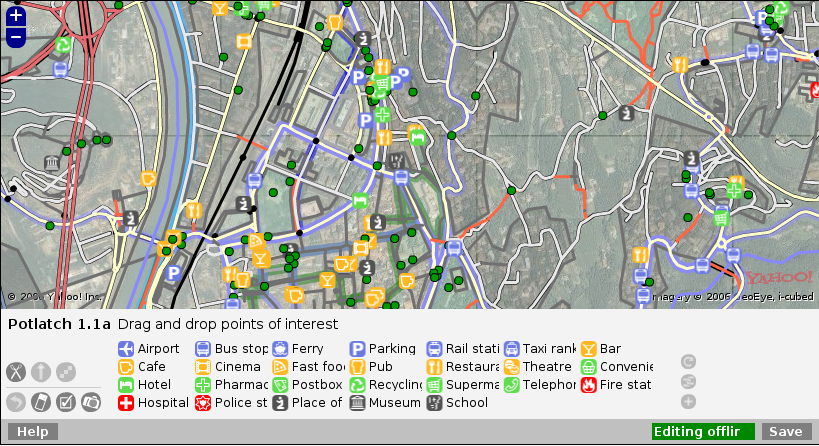
\includegraphics[width=0.7\columnwidth]{potlatch.png}
 \caption{\textit{L'interfaccia di \soft{Potlatch}}}
\end{wrapfloat}
Puoi collaborare alla mappatura anche se non hai il \gps, l'\textbf{importante è avere una connessione ad internet} \dots Come? Per esempio inserendo i nomi delle vie dove non sono presenti, inserendo i punti di interesse (negozi, punti turistici, fontane, servizi\dots), correggendo eventuali errori. Per molte zone si hanno le foto aeree di Yahoo in alta risoluzione, la cui licenza permette di "ricalcarle"; inoltre è stata concessa la possibilità di utilizzare le foto aeree disponibili sul Portale Cartografico Nazionale, distribute tramite servizi online WMS (Web Map Server), per derivare dati per il progetto \osm (si può fare solo con \soft{JOSM} o \soft{Merkator}). 

Se non hai un \gps potresti prendere in considerazione \soft{Walking Papers}, questo permette di stampare una zona e poi segnare su questa le modifiche da fare. Ovviamente si può usare questo strumento dove sono presenti un po' di dati sul database da utilizzare come base ed è molto utile per aggiungere waypoint nei centri. Per sfruttare al meglio il foglio modificato è bene avere uno scanner per importarlo nel PC e utilizzarlo con altri software, in primis \soft{JOSM}

\textbf{Preferisci sempre il sopralluogo di persona sul posto. Nel dubbio non mappare.}
\subsection{Ho il \gps}
Come spiegato nei primi paragrafi, le tracce \gps non entrano direttamente nel database di \osm. Sono però estremamente utili come base su cui ricalcare le way e i nodi mediante i software a disposizione, come \soft{Potlatch} o \soft{JOSM}.
\begin{wrapfloat}{figure}{L}{0pt}
 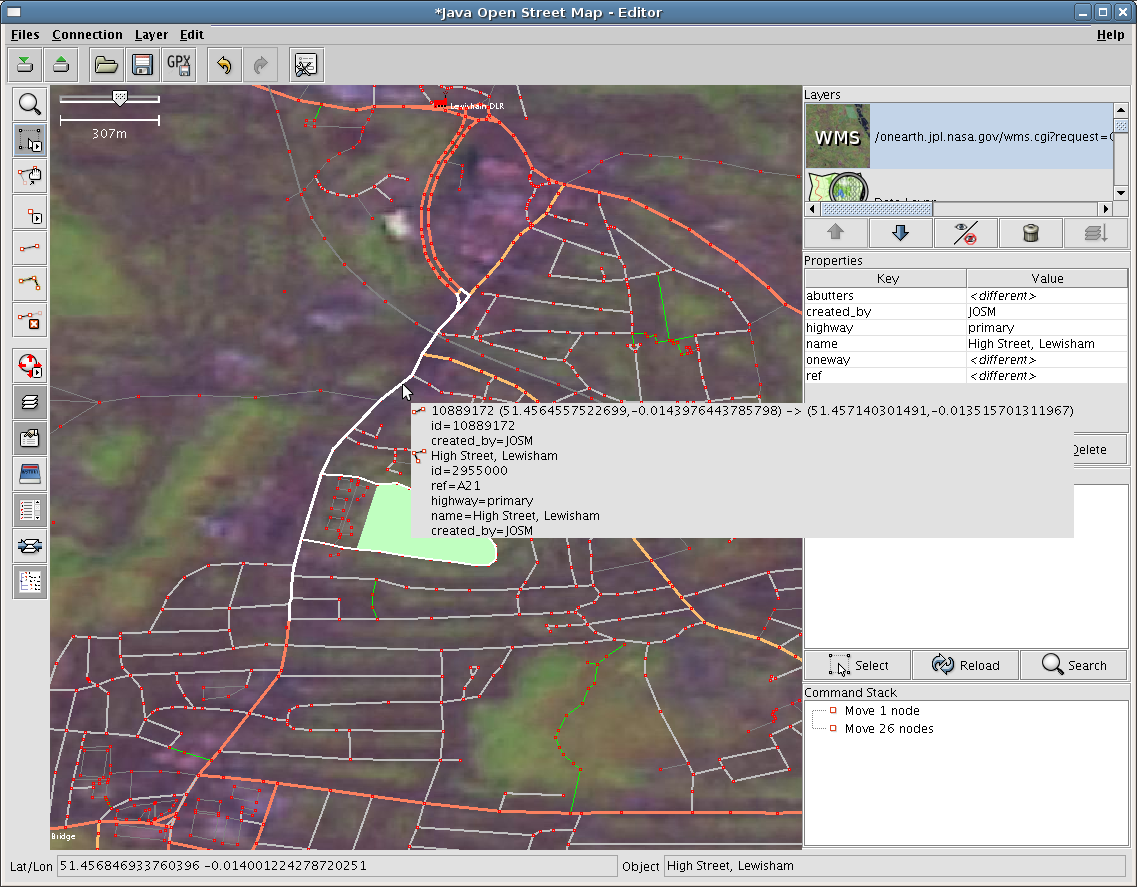
\includegraphics[width=0.6\columnwidth]{Josm-screenshot.png}
 \caption{\textit{L'interfaccia di JOSM}}
\end{wrapfloat}
Supponiamo di aver a disposizione un \gps per fare una bellissima gita in montagna. Accendiamo il nostro apparecchio, attendiamo l'aggancio dei satelliti ed iniziamo la registrazione della traccia. Per il progetto è molto importante avere i punti delle tracce abbastanza ravvicinati perciò \textbf{è bene settare nelle impostazioni del vostro \gps il salvataggio i punti delle tracce con una frequenza maggiore a quella di default}. Le impostazioni più utilizzate sono quelle basate sul \textit{tempo} (questo metodo va settato in base al mezzo di locomozione: in macchina e in bici vanno bene valori inferiori a 5 secondi; a piedi, con un passo non troppo svelto, si può arrivare fino a 10) oppure sulla \textit{distanza} (in questo caso è bene non superare i 10 m, sui garmin è il minimo disponibile), per i novizi è consigliato di utilizzare la distanza poichè questo metodo crea una traccia ``più pulita'' rispetto al metodo del tempo.

Il nostro percorso inizia su una strada forestale. È bene in questo caso appuntare questa informazione poiché nella fase di editing sarà importante per etichettarla correttamente con \key{highway}=\val{track}. Un modo semplice per tener nota di queste cose è utilizzare i waypoint registrabili col \gps, cioè memorizzare nel nostro caso il punto di inizio della strada forestale con un waypoint e, se il modello lo permette, assegnargli un nome significativo (es. inizio forestale). Se il \gps non lo permette appuntare su un pezzo di carta il codice del waypoint in questione e la sua descrizione. Allo stesso modo registreremo la fine della strada forestale con un altro waypoint, così come l'inizio del sentiero.

Sempre mediante i waypoint, è utile appuntare informazioni interessanti come il codice del sentiero o il suo nome.

È da precisare che il nome che si assegna ai waypoint non è fondamentale, ma serve come promemoria personale, infatti nemmeno i waypoint entrano a far parte del database di OSM, ma serviranno esclusivamente da appunti in fase di editing. Adottate quindi lo stile che più trovate utile, completo e comodo per appuntare quel che trovate.

Un altro metodo utilizzato è quello di sfruttare le potenzialità di un registratore digitale e \soft{JOSM}, infatti quest'ultimo software permette di sincronizzare la vostra traccia \gps con la registrazione audio. Sono due le possibilità di utilizzo del registratore, la prima è di accendere il registratore in concomitanza dell'inizio della registrazione della traccia \gps e lasciar-lo acceso; bisogna ricordarsi di prendere un waypoint per ogni elemento registrato vocalmente in modo tale da potersi spostare facilmente da un punto ad un altro; questa metodologia può essere molto comoda quando si è alla guida di un mezzo di trasporto tipo bicicletta o automobile. L'altra possibilità è quella di accendere il registratore solo in concomitanza della mappatura di un waypoint.

Ovviamente non solo le strade sono importanti per \osm: ad esempio nel nostro giro in montagna potrebbe essere interessante avere a disposizione segnavia (\key{turism}=\val{information} \& \key{information}=\val{guidepost}), bivacchi (\key{amenity}=\val{shelter}), rifugi (\key{tourism}=\val{alpine\_hut}), fontane d'acqua potabile (\key{amenity}=\val{drinking\_water}) e molto altro ancora.

A questo punto, giunti a casa dalla nostra gita, scarichiamo sul PC le tracce e i waypoints rilevati, apriamo il nostro editor preferito e dal menù carichiamo sia le tracce che i waypoints che quindi ci appariranno sullo schermo. Ora si possono scaricare i dati di \osm già presenti sul server mediante l'apposito pulsante.

Attraverso i tool di disegno si vanno così a ricalcare le nostre tracce assegnando i tag di descrizione; le modifiche effettuate possono ora essere caricate sul server di \osm mediante l'apposito pulsante.

Sulla mappa in homepage (detta slippy map) le modifiche non appariranno istantaneamente ma si dovrà attendere un po' di tempo prima che vengano renderizzate; questo processo può durare pochi minuti così come qualche giorno.

È da sottolineare che le tracce pur non entrando direttamente nel data-base principale di \osm, è possibile caricarle sul sito tramite la pagina \url{http://www.openstreetmap.org/traces}, al fine di renderle pubbliche e disponibili a chiunque le voglia ricalcare o controllare; inoltre, passando più volte nella stessa ``strada'', avremo delle tracce sempre un po' diverse, avendone tante si può avere una precisione maggiore facendo passare la nostra way nella linea mediana di tutte le tracce.
\subsection{Ho un cellulare con \gps integrato o collegabile ad un'antenna \gps}
Il continuo sviluppo tecnologico ha portato alla costruzione di cellulari sempre più complessi e performanti; molti modelli delle ultime generazioni hanno un ricevitore \gps incorporato, questa situazione ha fatto si che venissero sviluppati programmi per contribuire al progetto e per visualizzare/utilizzare i dati di \osm. Esistono software per la maggiorparte dei sistemi operativi (Linux, Android, Symbian, Windows CE) utilizzati sui cellulari. Nella sezione software vengono presentati alcuni dei più utilizzati.

\subsection{Infine...}
Molto altro ci sarebbe da dire, inizia pure a lavorare con cautela e \textbf{per qualsiasi dubbio, domanda in mailing list o sul canale irc. Prima di chiedere controlla che qualcuno non abbia già avuto il tuo stesso problema consultando gli archivi della mailing list}.

\textbf{MOLTO IMPORTANTE: non copiare mai da altre mappe se non sei sicuro di poterlo fare. Né Google né le carte topografiche hanno una licenza che ne permette la copia}.

\section{Donazione tracce}
Se hai delle tracce \gps da te registrate e non hai voglia o tempo di imparare a importarle, puoi aiutare \osm già da subito "donandole".

Qualcuno della comunità, possibilmente che conoscerà la tua zona, le caricherà all'interno del database di \osm.

Le tracce migliori sono quelle su un unico tipo di percorso, ad es. tutto sentiero o tutto strada forestale , ma anche le altre in generale vanno bene; in questo caso sarebbe meglio avere un minimo di conoscenza della zona oppure una breve descrizione del tracciato. Ricordati: \textbf{togli l'opzione di seguire fedelmente il tracciato preesistente}.
\section{Passaparola}
Se a te il progetto non interessa, \textbf{passaparola a tutti coloro che potrebbero essere incuriositi o che potrebbero dare una mano}.

Quando c'è la possibilità, usa le mappe online di \osm, se hai da mostrare delle zone a degli amici, ma usale anche nei forum e nel resto del web; integrarle col vostro sito risulterà molto facile. %INSERIRE CODICE PER INSERIRLE.
 
In alcune zone il dettaglio e la grafica sono molto superiori ad altre alternative.
\section{Mapping party}
\begin{wrapfloat}{figure}{L}{0pt}
 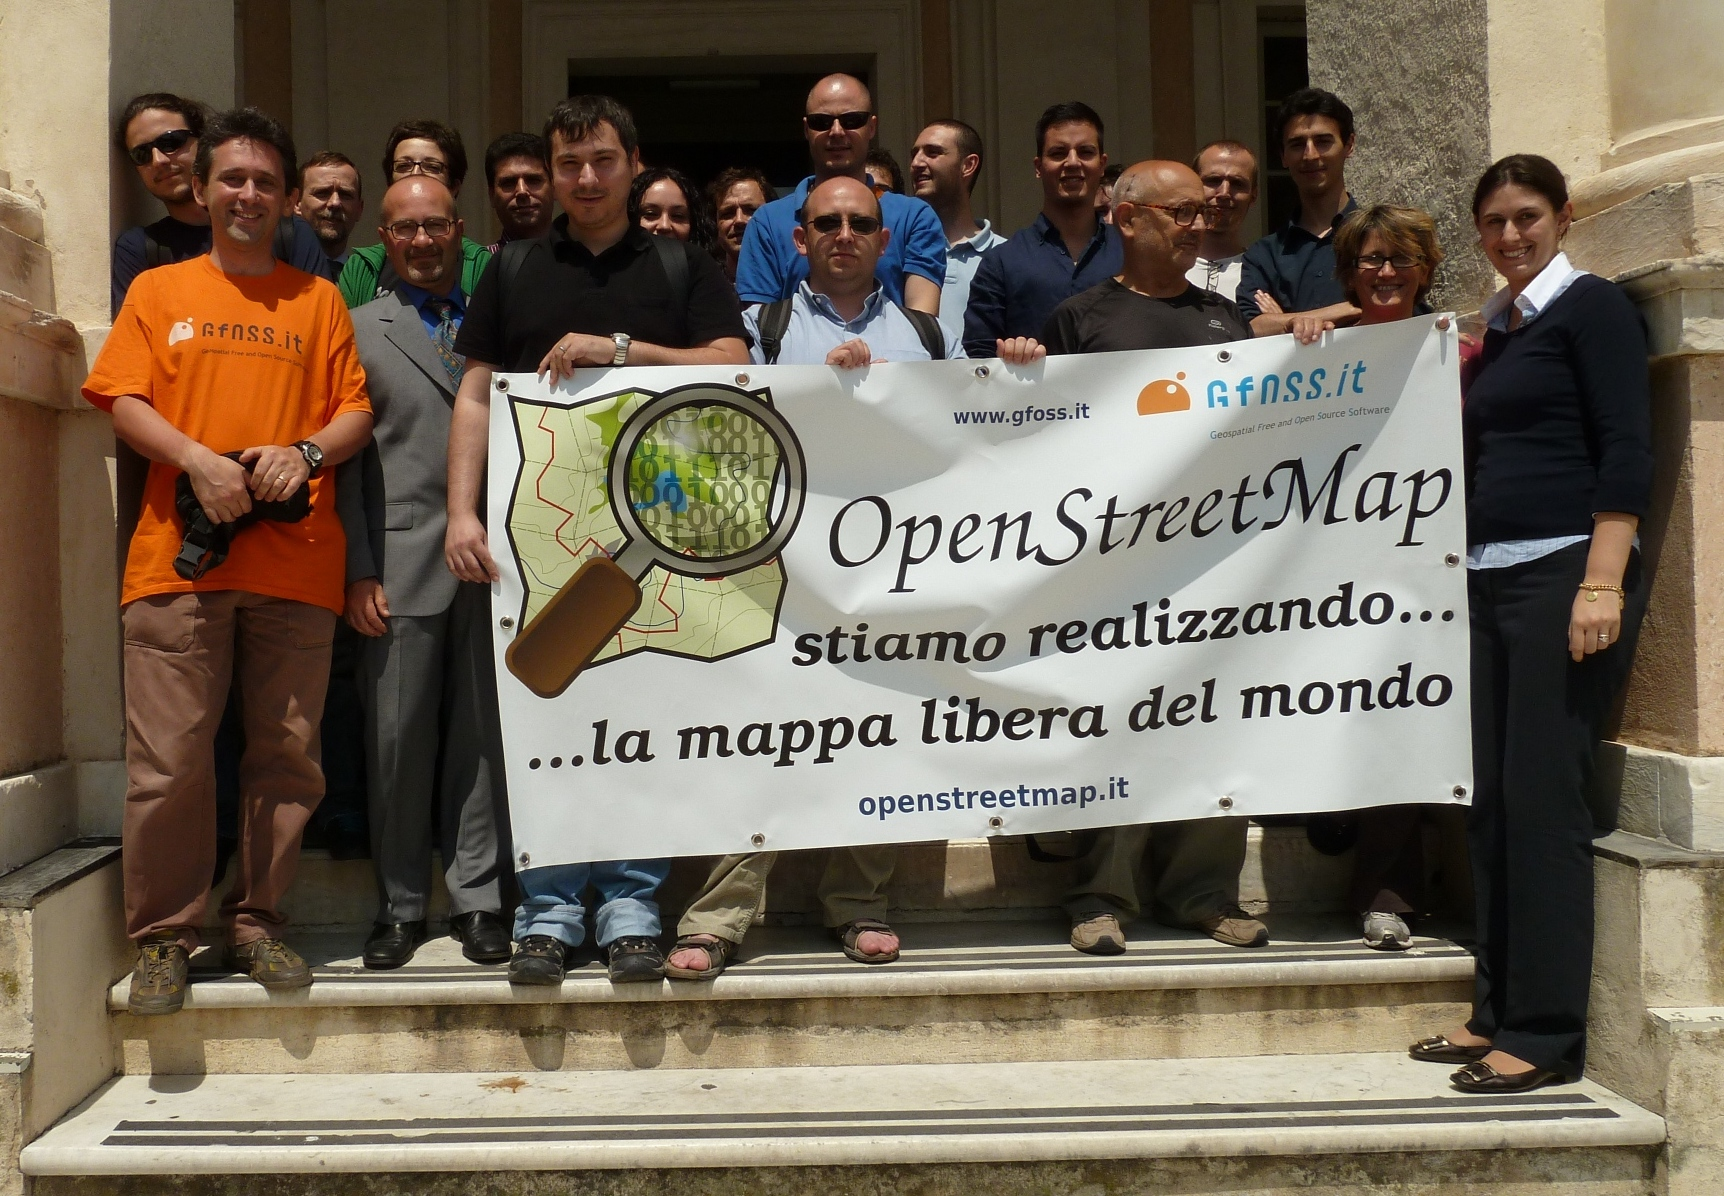
\includegraphics[width=0.55\columnwidth]{Osmit2010.JPG}
 \caption{\small{\textit{La foto di gruppo di OSMit 2010}}}
\end{wrapfloat}
I \textbf{mapping party sono eventi legati al progetto}, durante i quali un certo numero di OSMapper, così è chiamato chi partecipa a \osm, sceglie una zona, solitamente poco mappata oppure da completare, incomincia a pubblicizzare l'evento all'interno della comunità e all'esterno contattando enti pubblici, associazioni e media per diffondere la manifestazione. Il contatto esterno alla comunità è molto importante per cercare di coinvolgere nuove persone all'interno del progetto.

Solitamente i mapping party si tengono nel corso del weekend per cercare di far affluire più persone possibili; ricordo tra gli altri, il Mapping Party di Arezzo, il primo ufficiale in Italia, quello di Pompei, con scopi archeologici all'interno dei resti romani della nota località napoletana, M(')appare Portofino, per la sentieristica del Parco naturale regionale di Portofino, Dolomiti Mapping Party e il Graian Alps Mapping Party; anche questi ultimi due avevano un tema specifico: la montagna; il primo tra il gruppo del Brenta e il secondo, effettuato grazie al supporto del Parco Nazionale del Gran Paradiso, nella valle dell'Orco in Piemonte.

Inoltre \textbf{si possono realizzare anche eventi di durata minore, i micro mapping party} (Roma, Vicenza, Trentino, Milano). In Italia abbiamo anche sperimentato, con ottimi risultati, un mapping party dilatato nei mesi: M(')appare Milano. Con il supporto della trasmissione radiofonica Mentelocale trasmessa su Radio Popolare di Milano e dell'associazione di volontariato \pro{GFOSS.it}, sono stati organizzati per tre mesi micro mapping party con cadenza bisettimanale, questo ha permesso di andare a coprire molte zone del capoluogo lombardo e di diffondere il progetto. Da due anni si tiene un evento nazionale su \osm denominato OSMit, la prima edizione si è tenuta a Trento la seconda a Genova.
\section{Humanitarian OpenStreetMap Team}
L'\pro{Humanitarian OpenStreetMap Team (HOT)} è un gruppo di OSMapper che hanno creato un ``team'' per utilizzare il progetto per scopi ``uma-nitari''.

La prima volta che \osm è stato utilizzato per queste finalità è evvenuto alla ripresa delle ostilità tra Israele e Palestina nel 2009, la comunità si è autofinanziata per acquistare le ortofoto recenti della Striscia di Gaza in modo tale da poter digitalizzare i dati.

Il caso più eclatante, invece, è stato in concomitanza di una delle più grandi catastrofi naturali negli ultimi anni, il terremoto ad Haiti. In questa occasione Google ha sovvenzionato l'acquisto delle ortofoto della situazione post terremoto, e gli utenti hanno provveduto celermente alla digitalizzazione, segnalando tra le altre cose la presenza di campi di soccorso, i ponti distrutti e altri elementi utili ai soccoritori; inoltre sono stati messi in piedi diversi servizi per fare in modo che si potessero utilizzare facilmente i dati presenti sul database aggiornati quasi in tempo reale, vi era la possibilità di trovarli in formato garmin (per gli operatori che si dovevano spostare da un posto all'altro), in formato immagine per essere stampata (per coordinare gli aiuti dai campi di soccorso) inoltre erano presenti diversi siti online che avevano creato strati informativi dedicati all'isola caraibica. Questa tragica esperienza ha mostrato al mondo come \osm possa essere utile, ha mostrato come \textit{i dati creati dal basso} sono in certi casi essenziali, non a caso erano gli unici aggiornati al post terremoto e utilizzabili durante la situazione di emergenza.

Altro progetto molto interessate è riguardante uno dei più grande slum dell'Africa: Kibera.
Questa località per i grandi vendor di dati geografici non esiste ma in realtà conta circa un milione di persone. Qui è stato realizzato un qualcosa di più complesso, alcuni componenti di \pro{HOT} si sono recati nella ``città'' africana e hanno istruito diversi abitanti del luogo, facendo capire a cosa serve il progetto e come partecipare. Ad oggi i dati presenti sul database di \osm sono sicuramente la migliore fonte cartografica della zona.
\section{Informazioni utili}
\textbf{\url{http://wiki.openstreetmap.org/wiki/WikiProject_Italy} è il portale principale della comunità italiana}, per vedere il lavoro a livello nazionale e contattare gli altri utenti della penisola. È molto utile contribuire sul wiki attraverso \textbf{traduzioni} di pagine già esistenti in altre lingue, che servono sempre sia ai nuovi arrivati che a quelli che non conoscono al meglio la lingua inglese (la più usata sul wiki insieme al tedesco), sia alla \textbf{creazione e al mantenimento delle pagine} in italiano oltre a quelle della vostra regione, provincia o comune.

Esiste anche un sito in italiano che in questo momento è in fase di sviluppo \url{http://www.openstreetmap.it}; attualmente l'unica parte attiva è il blog \url{blog.openstreetmap.it}.

Tieni costantemente sotto controllo anche il portale wiki internazionale \url{http://wiki.openstreetmap.org/wiki/Main_Page} che contiene sempre ottimi spunti.  La comunità più attiva è quella tedesca con una marea di volontari. In Italia il progetto è iniziato nel 2007 ed ora incomincia ad essere utilizzabile in special modo a livello locale e non globale poichè vi sono zone molto ben mappate e altre ancora vuote.

Se hai dubbi o domande consulta le risposte alle domande frequenti \url{http://wiki.openstreetmap.org/index.php/It:FAQ}, altri potrebbero aver avuto il tuo stesso problema e potresti trovare la soluzione.
\section{Contatti}
\textbf{Il principale riferimento nazionale è la mailing list italiana:\newline \url{http://lists.openstreetmap.org/listinfo/talk-it}}

Altra risorsa utile è la chat (canale irc) \#osm-it @ irc.oftc.net, che può essere raggiunta, oltre che da client irc, anche attraverso questo indirizzo web \url{https://www.mibbit.com/?server=irc.oftc.net\&channel=\%23osm-it}; ci puoi trovare anche nella chat (canale irc) di \pro{GFOSS.it}, la principale associazione che supporta OSM in Italia, l'indirizzo è \#gfoss @ irc.eu.freenode.net. Ci suò accedere anche via web tramite \url{webchat.freenode.net}  canale \#gfoss

Esistono inoltre molti strumenti internazionali per svariate notizie su \osm \url{http://wiki.openstreetmap.org/wiki/Mailing_list}

\section{Software}
Di seguito verranno segnalati software, con diverse finalità, che hanno la possibilità di interfacciarsi con \osm.

\subsection{Editor}
\soft{JOSM}: l'editor per \osm più utilizzato, scritto in Java ha molti tools utilissimi oltre a svariati plugin

\soft{Potlach}: editor online dal sito principale di \osm, molto comodo per la possibilità di avere le foto aeree di Yahoo come sfondo

\soft{Merkator}: altro editor per \osm

\subsection{Qualità}
Di seguito sono riportati solo alcuni degli strumenti, per avere una visione completa dei programmi per mantenere alta la qualità dei dati in \osm controllate questa pagina \url{http://wiki.openstreetmap.org/wiki/IT:Quality_Assurance}

\soft{OpenStreetBugs}: uno dei primi strumenti per la qualità dei dati, permette agli utenti di segnalare errori

\soft{QualityStreetMap}: permette di segnalare le zone completamente mappate attraverso griglie per diversi tag, copre tutta Europa

\soft{Keep Right}: segnala diverse tipologie di errore

\subsection{Analisi}
\soft{Osmosis}: programma per gestire i dati di \osm

\soft{QGIS}: software GIS per l'analisi e la visualizzazione di dati geografici, si interfaccia con \osm attraverso diversi tool che permettono lo scaricamento, la modifica e l'aggiornamento del database

\soft{PostgreSQL/PostGIS}: database relazionale che con la sua estensione spaziale PostGIS può contenere i dati di \osm caricati utilizzando il software osm2pgsql

\soft{PgRouting}: estensione di PostGIS per effettuare calcoli di routing; esiste osm2pgrouting che importa i file di \osm in PostgreSQL con le tabelle conformi al formato richiesto da PgRouting

\soft{Spatialite}: estensione spaziale del database Sqlite; attraverso il mo-dulo spatialite\_osm carica file .osm; al suo interno è implementanto un ottimo algoritmo per il routing 

\subsection{Rendering}

\soft{Mapnik}: software per la rappresentazione di dati geografici, può creare singole immagini o tile per la pubblicazione sul web

\soft{Osmarender}: simile al precedente

\soft{Maperitive}: simile al precedente, molto user friendly

\soft{MapOSMatic}: a differenza dei precedenti permette di stampare, con uno stile predefinito una mappa a grande scala e lo stradario

\subsection{Visualizzatori}

\soft{Navit}: software per il routing con i dati di \osm, esistono versioni per diverse piattaforme, compresi cellulari

\soft{OpenLayers}: client WebGIS che permette di visualizzare in modo molto semplice le tile di \osm

\soft{Marble}: visualizzatore di dati geografici su modello Google Earth

\soft{OSM3D}: visualizzatore 3D per i dati \osm

\subsection{GPS}

\soft{Qlandkarte}: software utilizzato soprattutto per la visualizzazione e la gestione di dati scaricati dal \gps, permette la visualizzazione come sfondo delle mappe di OSM

\soft{MkGmap}: trasforma i dati in formato .osm in formato .img per Garmin

\soft{Groudtruth}: simile al precedente

\subsection{Cellulari}
\subsubsection{Android}

\soft{Vespucci}: un buon editor, non è a livello di JOSM ma è comunque uno strumento molto valido per uno smartphone

\soft{OSMtracker}: editor con possibilità di mappe offline (esiste una versione anche per windows mobile)

\soft{Mapdroyd}: visualizzatore di mappe offline
\subsubsection{IPhone/IPad}

\soft{Mapzen Poi Collector}: editor solamente puntuale

\soft{OSMTrack}: serve per registrare tracce
\subsubsection{N900/Maemo}

\soft{osm2go}: editor molto buono che interagisce - runtime - con il server di \osm
\subsubsection{java2me}

\soft{GpsMid}: carica mappe vettoriali di \osm e permette di creare POI e tracce

\section{Link}
\subsection{Visualizzazione}
\url{http://www.openstreetmap.org}: è il portale ufficiale di OSM. Da qui potrai consultare le mappe dimostrative “ufficiali” cliccando sul + in alto a destra sulla mappa:
Mapnik e Osmarender sono mappe generiche che mostrano molte caratteristiche mappate,
Cyclemap è invece una mappa tematica pensata per i ciclisti. Evidenzia le piste ciclabili nazionali, regio-nali e locali (ove mappate logicamente), le fontanelle di acqua potabile, i negozi di bici, le curve di livello e una colorazione pensata per mettere in risalto i rilievi

\url{http://www.opencyclemap.org}: è il sito ufficiale della mappa sopra descritta

Di seguito una serie di link che rappresentano sentieristica, mountain bike:
\begin{itemize}
 \item \url{http://www.wanderreitkarte.de/}
 \item \url{http://maps.refuges.info/}
 \item \url{http://hikebikemap.de/}
 \item \url{http://beta.letuffe.org/?layers=00B00FFFFFFFFFFFFF}
 \item \url{http://osm.lonvia.de/world_hiking.html}
\end{itemize}

\url{http://www.openpistemap.org}: è una mappa tematica pensata per gli amanti degli sport invernali, vengono renderizzati gli impianti di risalita, le piste a seconda della scala di difficoltà e le isolinee

\url{http://whitewater.quaker.eu.org/}: mappa tematica per l'attività sportiva lungo i fiumi

\url{http://www.openseamap.org}: mappa tematica che visualizza gli elementi utili alla navigazione

\url{http://3liz.fr/public/osmtransport/}: mappa che visualizza i tra-sporti pubblici, è possibile interrogare gli elementi per avere maggiori informazioni

\url{http://openbusmap.org/}: altro visualizzatore di trasporti pubblici

\url{http://toolserver.org/~stephankn/cuisine/}: è una mappa tema-tica dedicata alle diverse tipologie di ristoranti

\url{http://toolserver.org/~ti/distance-o-meter/}: strumento molto interessante che permette di visualizzare la copertura di diversi elementi puntuali attraverso buffer

\url{http://www.openstreetbrowser.org}: permette di visualizzare innumerevoli informazioni inserite in \osm, altrimenti nascoste o vi-sibili soltanto mediante un rendering ad hoc. Ne sono un esempio l'evidenziamento dinamico dei percorsi dei mezzi pubblici con le relative fermate, ma anche strutture turistiche, storiche, sportive

\url{http://www.yournavigation.org}: si tratta di un navigatore che permette di trovare il percorso migliore che unisce due punti. È possibile scegliere il più breve, il più veloce o l'utilizzo a piedi o in bicicletta. I percorsi trovati per la bici daranno priorità alle piste ciclabili

\url{http://www.openrouteservice.org}: il servizio principale proposto è un navigatore simile a quello sopra descritto. In Germania, basandosi sul servizio strade è capace di calcolare in tempo reale il percorso migliore in base al traffico od eventuali incidenti. Il sito fornisce inoltre servizi più specifici come ad esempio il tempo di accessibilità: dato un punto sulla mappa verrà evidenziata l'area raggiungibile entro un determinato tempo dal punto considerato

\url{http://www.openaddresses.org/}: visualizza e permette di inserire indirizzi di civici

\url{http://oobrien.com/oom/?layers=B00FFTF}: OpenOrienteeringMap, mappa libera per l'orienteering

\url{http://tagwatch.stoecker.eu/}: informazioni sull'utilizzo dei tag

\url{http://taginfo.openstreetmap.de/}: come sopra

\subsection{Servizi}

\url{http://www.itoworld.com}: è un'azienda che fornisce un utile servizio per verificare l'attività di mappatura in una determinata zona: scoprire  e contattare gli utenti che ci lavorano, vedere le modifiche nel tempo. Necessita di registrazione gratuita

\url{http://www.cloudmade.com}: fornisce svariati servizi come ad esempio, previa registrazione, la possibilità di creare in modo semplice mappe con rendering personalizzato

\url{http://www.geofabrik.de}: fornisce svariati servizi come la possibilità di scaricare i dati osm relativi ad una determinata nazione e un tool per confrontare le mappe \osm con le mappe di google. Si scoprirà come in molti casi la precisione e il dettaglio di osm siano superio-ri a googlemaps. Le mappe di google devono essere utilizzate solo come interessante confronto e non per essere copiate

\url{http://walking-papers.org}: permette di stampare una mappa da utilizzare durante le ``mappature'' per segnare nuovi elementi, inoltre una volta scannerizzato il foglio con le modifiche si può inserire sul portale

\url{http://download.gfoss.it/osm/}: distribuisce i file italiani di \osm in diversi formati: backup del file italiano e file .osm diviso per regioni, .img per Garmin e formato per \soft{Navit}

\url{http://www.gfoss.it/osm/stat/}: statistiche e stradario diviso per limiti amministrativi

\vfill
\begin{center}\begin{small}\textbf{
Questo documento è rilasciato con licenza 
Creative Commons Attribuzione - Non commerciale - Condividi allo stesso modo
\url{http://creativecommons.org/licenses/by-nc-sa/2.5/it/}}\end{small}\end{center}
\begin{center}
 
\includegraphics{ccbysa.png}
\end{center}
\end{document}
